\documentclass{beamer}
\mode<presentation>
\usepackage{amsmath,amssymb,mathtools}
\usepackage{textcomp}
\usepackage{gensymb}
\usepackage{adjustbox}
\usepackage{subcaption}
\usepackage{enumitem}
\usepackage{multicol}
\usepackage{listings}
\usepackage{url}
\usepackage{graphicx} % <-- needed for images
\def\UrlBreaks{\do\/\do-}

\usetheme{Boadilla}
\usecolortheme{lily}
\setbeamertemplate{footline}{
  \leavevmode%
  \hbox{%
  \begin{beamercolorbox}[wd=\paperwidth,ht=2ex,dp=1ex,right]{author in head/foot}%
    \insertframenumber{} / \inserttotalframenumber\hspace*{2ex}
  \end{beamercolorbox}}%
  \vskip0pt%
}
\setbeamertemplate{navigation symbols}{}

\lstset{
  frame=single,
  breaklines=true,
  columns=fullflexible,
  basicstyle=\ttfamily\tiny   % tiny font so code fits
}

\numberwithin{equation}{section}

% ---- your macros ----
\providecommand{\nCr}[2]{\,^{#1}C_{#2}}
\providecommand{\nPr}[2]{\,^{#1}P_{#2}}
\providecommand{\mbf}{\mathbf}
\providecommand{\pr}[1]{\ensuremath{\Pr\left(#1\right)}}
\providecommand{\qfunc}[1]{\ensuremath{Q\left(#1\right)}}
\providecommand{\sbrak}[1]{\ensuremath{{}\left[#1\right]}}
\providecommand{\lsbrak}[1]{\ensuremath{{}\left[#1\right.}}
\providecommand{\rsbrak}[1]{\ensuremath{\left.#1\right]}}
\providecommand{\brak}[1]{\ensuremath{\left(#1\right)}}
\providecommand{\lbrak}[1]{\ensuremath{\left(#1\right.}}
\providecommand{\rbrak}[1]{\ensuremath{\left.#1\right)}}
\providecommand{\cbrak}[1]{\ensuremath{\left\{#1\right\}}}
\providecommand{\lcbrak}[1]{\ensuremath{\left\{#1\right.}}
\providecommand{\rcbrak}[1]{\ensuremath{\left.#1\right\}}}
\theoremstyle{remark}
\newtheorem{rem}{Remark}
\newcommand{\sgn}{\mathop{\mathrm{sgn}}}
\providecommand{\abs}[1]{\left\vert#1\right\vert}
\providecommand{\res}[1]{\Res\displaylimits_{#1}}
\providecommand{\norm}[1]{\lVert#1\rVert}
\providecommand{\mtx}[1]{\mathbf{#1}}
\providecommand{\mean}[1]{E\left[ #1 \right]}
\providecommand{\fourier}{\overset{\mathcal{F}}{ \rightleftharpoons}}
\providecommand{\system}{\overset{\mathcal{H}}{ \longleftrightarrow}}
\providecommand{\dec}[2]{\ensuremath{\overset{#1}{\underset{#2}{\gtrless}}}}
\newcommand{\myvec}[1]{\ensuremath{\begin{pmatrix}#1\end{pmatrix}}}
\let\vec\mathbf

\title{MatGeo Presentation - Problem 12.389}
\author{EE25BTECH11064 - Yojit Manral}
\date{}

\begin{document}

\frame{\titlepage}
\begin{frame}{Question}
\begin{align*}
    x + 2y + z = 4 \\
    2x + y + 2z = 5 \\
    x - y + z = 1
\end{align*}
The system of algebraic equations given above has
\begin{enumerate}[label=(\alph*)]
    \item a unique solution of $(x = 1, y = 1, z = 1)$.
    \item only the two solutions of $(x = 1, y = 1, z = 1)$ and $(x = 2, y = 1, z = 0)$.
    \item infinite number of solutions.
    \item no feasible solution.
\end{enumerate}
\end{frame}

\begin{frame}{Solution}
$\rightarrow$ The above equations can be written in matrix form as
\begin{align}
    \myvec{1&2&1\\2&1&2\\1&-1&1}\myvec{x\\y\\z} &= \myvec{4\\5\\1} \\
    \vec{A} \hspace{0.95cm} \vec{x} \hspace{0.12cm} &= \hspace{0.12cm} \vec{B}
\end{align}
$\rightarrow$ Using the augmented matrix $\brak{\vec{A}|\vec{B}}$
\begin{align}
    \brak{\begin{array}{ccc|c}1&2&1&4\\2&1&2&5\\1&-1&1&1\end{array}}
    \xrightarrow[R_3 \leftrightarrow R_3 - R_1]{R_2 \leftrightarrow R_2 - 2R_3} \brak{\begin{array}{ccc|c}1&2&1&4\\0&3&0&3\\0&-3&0&-3\end{array}} \\
    \xrightarrow[R_1 \leftrightarrow R_1 - (2/3)R_2]{R_3 \leftrightarrow R_3 + R_2}
    \brak{\begin{array}{ccc|c}1&0&1&2\\0&3&0&3\\0&0&0&0\end{array}} \\
    \implies x + z = 2 \text{ and } y = 1
\end{align}
$\rightarrow$ So, the system of equations has infinite solutions given by the intersection of the planes $x + z = 2$ and $y = 1$. \\
\end{frame}

\begin{frame}{Solution}
$\rightarrow$ Therefore, \textit{(c) infinite number of solutions.} is the correct option.
\begin{figure}[h!]
   \centering
   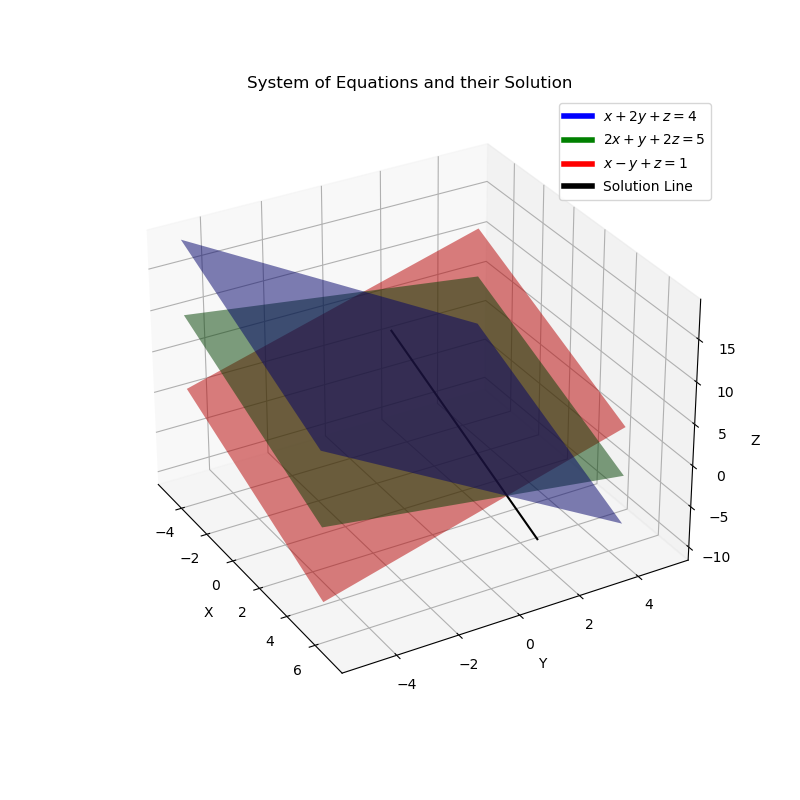
\includegraphics[width=0.6\linewidth]{figs/01.png}
   \caption{Plot of system of equations and solution line}
   \label{Plot_1}
\end{figure}
\end{frame}
 % --------- CODE APPENDIX ---------
\section*{Appendix: Code}

% C program
\begin{frame}[fragile]{File: points.c}
\begin{lstlisting}[language=C]
#include <stdio.h>

int main() {
  FILE *fp;

  // -------------------
  // Question 12.389
  // -------------------


  fp = fopen("points.dat", "w");
  fprintf(fp, "%d,%d,%d,%d\n", 1, 2, 1, 4); // 1
  fprintf(fp, "%d,%d,%d,%d\n", 2, 1, 2, 5); // 2
  fprintf(fp, "%d,%d,%d,%d\n", 1, -1, 1, 1); // 3
  fclose(fp);
  return 0;
}
\end{lstlisting}
\end{frame}

% Python calling C
\begin{frame}[fragile]{File: call\_c.py}
\begin{lstlisting}[language=Python]
import subprocess

# Compile the C program
subprocess.run(["gcc", "points.c", "-o", "points"])

# Run the compiled C program
result = subprocess.run(["./points"], capture_output=True, text=True)

# Print the output from the C program
print(result.stdout)
\end{lstlisting}
\end{frame}

% Python plotting
\begin{frame}[fragile]{File: plot.py}
\begin{lstlisting}[language=Python]
import numpy as np
import matplotlib.pyplot as plt
from mpl_toolkits.mplot3d import Axes3D
from matplotlib.lines import Line2D

# Define the equations
def plane1(x, y):
    return 4 - x - 2 * y

def plane2(x, y):
    return (5 - 2*x - y) / 2

def plane3(x, y):
    return 1 - x + y

# Create meshgrid for x and y
x_vals = np.linspace(-5, 5, 10)
y_vals = np.linspace(-5, 5, 10)
X, Y = np.meshgrid(x_vals, y_vals)

# Compute Z values for each plane
Z1 = plane1(X, Y)
Z2 = plane2(X, Y)
Z3 = plane3(X, Y)

# Plotting the planes and solution
fig = plt.figure(figsize=(12, 8))
ax = fig.add_subplot(111, projection='3d')
\end{lstlisting}
\end{frame}

\begin{frame}[fragile]{File: plot.py}
\begin{lstlisting}[language=Python]

# Plot each plane
surf1 = ax.plot_surface(X, Y, Z1, color='blue', alpha=0.5, rstride=100, cstride=100)
surf2 = ax.plot_surface(X, Y, Z2, color='green', alpha=0.5, rstride=100, cstride=100)
surf3 = ax.plot_surface(X, Y, Z3, color='red', alpha=0.5, rstride=100, cstride=100)

# Plot the solution line (x = 2 - z, y = 1)
z_vals = np.linspace(-5, 5, 10)
x_sol = 2 - z_vals
y_sol = np.ones_like(z_vals)

line = ax.plot(x_sol, y_sol, z_vals, color='black', label='Solution Line')

# Labels
ax.set_xlabel('X')
ax.set_ylabel('Y')
ax.set_zlabel('Z')

ax.set_title('System of Equations and their Solution')

# Manually add legend
ax.legend(handles=[
    Line2D([0], [0], color='blue', lw=4, label=r'$x + 2y + z = 4$'),
    Line2D([0], [0], color='green', lw=4, label=r'$2x + y + 2z = 5$'),
    Line2D([0], [0], color='red', lw=4, label=r'$x - y + z = 1$'),
    Line2D([0], [0], color='black', lw=4, label='Solution Line')
])

# Show the plot
ax.view_init(30, -30)
plt.show()
\end{lstlisting}
\end{frame}

\end{document}
